%% LyX 2.2.0 created this file.  For more info, see http://www.lyx.org/.
%% Do not edit unless you really know what you are doing.
\documentclass[english]{beamer}
\usepackage[T1]{fontenc}
\usepackage[latin9]{inputenc}
\setcounter{secnumdepth}{3}
\setcounter{tocdepth}{3}
\usepackage{babel}
\usepackage{calc}
\usepackage{graphicx}
\ifx\hypersetup\undefined
  \AtBeginDocument{%
    \hypersetup{unicode=true,pdfusetitle,
 bookmarks=true,bookmarksnumbered=false,bookmarksopen=false,
 breaklinks=false,pdfborder={0 0 1},backref=false,colorlinks=true}
  }
\else
  \hypersetup{unicode=true,pdfusetitle,
 bookmarks=true,bookmarksnumbered=false,bookmarksopen=false,
 breaklinks=false,pdfborder={0 0 1},backref=false,colorlinks=true}
\fi

\makeatletter

%%%%%%%%%%%%%%%%%%%%%%%%%%%%%% LyX specific LaTeX commands.
%% Because html converters don't know tabularnewline
\providecommand{\tabularnewline}{\\}

%%%%%%%%%%%%%%%%%%%%%%%%%%%%%% Textclass specific LaTeX commands.
 % this default might be overridden by plain title style
 \newcommand\makebeamertitle{\frame{\maketitle}}%
 % (ERT) argument for the TOC
 \AtBeginDocument{%
   \let\origtableofcontents=\tableofcontents
   \def\tableofcontents{\@ifnextchar[{\origtableofcontents}{\gobbletableofcontents}}
   \def\gobbletableofcontents#1{\origtableofcontents}
 }
 \newenvironment{lyxcode}
   {\par\begin{list}{}{
     \setlength{\rightmargin}{\leftmargin}
     \setlength{\listparindent}{0pt}% needed for AMS classes
     \raggedright
     \setlength{\itemsep}{0pt}
     \setlength{\parsep}{0pt}
     \normalfont\ttfamily}%
    \def\{{\char`\{}
    \def\}{\char`\}}
    \def\textasciitilde{\char`\~}
    \item[]}
   {\end{list}}

%%%%%%%%%%%%%%%%%%%%%%%%%%%%%% User specified LaTeX commands.
\usetheme[secheader]{Boadilla}
\usecolortheme{seahorse}
\title{Concurrent Join Calculus in Scala}
\author{Sergei Winitzki}
\date{November 11, 2016}
\institute[Workday, Inc.]{Scala by the Bay 2016}

\makeatother

\begin{document}
\frame{\titlepage}
\begin{frame}{What is ``Join Calculus''?}

``Join calculus'' is...
\begin{itemize}
\item ...a programming language for concurrent computations...
\item ...largely unknown and unused by the software engineering community 
\end{itemize}
\end{frame}

\begin{frame}{Parallelism vs.~Asynchrony vs.~Concurrency}


\framesubtitle{Parallelism}

Parallelism means...
\begin{itemize}
\item ...to use multithreading to speed up a \emph{sequential} computation
\begin{itemize}
\item main problem: to ``parallelize'' a computation efficiently
\end{itemize}
\item parallel collections, map/reduce, Spark
\end{itemize}
Typical task: count words in 10,000 text files
\end{frame}

\begin{frame}{Concurrency vs.~Parallelism vs.~Asynchrony}


\framesubtitle{Asynchrony}

Asynchrony means...
\begin{itemize}
\item ...to optimize \emph{sequential} computations that may have long wait
times
\begin{itemize}
\item main problem: to interleave wait times on a single-thread runloop
\end{itemize}
\item futures/promises, async/await, streams, FRP, coroutines
\end{itemize}
Typical task: implement interactive Excel tables with auto-updating
cells
\end{frame}

\begin{frame}{Concurrency vs.~Parallelism vs.~Asynchrony}


\framesubtitle{Concurrency}

Concurrency means...
\begin{itemize}
\item ...mutually interacting computations, running in unknown order
\begin{itemize}
\item main problem: to decide when to start a new process (or to wait)
\end{itemize}
\item \texttt{Thread}, \texttt{synchronized}, \texttt{semaphore}
\end{itemize}
Typical task: simulate ``dining philosophers''
\end{frame}

\begin{frame}{Dining philosophers}


\framesubtitle{The exemplary problem of concurrency}

\href{https://en.wikipedia.org/wiki/Dining_philosophers_problem}{Five philosophers sit at a round table},
taking turns eating and thinking for random time intervals
\begin{center}
\includegraphics[height=4cm]{An_illustration_of_the_dining_philosophers_problem}
\par\end{center}

Problem: run the process, avoiding deadlock and starvation
\end{frame}

\begin{frame}{Problems with concurrency}

Imperative concurrency is difficult to reason about:
\begin{itemize}
\item callbacks, threads, semaphores, mutexes, shared mutable state...
\item testing is hard \textendash{} non-deterministic runtime behavior!
\begin{itemize}
\item race conditions, deadlocks, livelocks
\end{itemize}
\end{itemize}
We try to \emph{avoid} concurrency whenever possible!
\end{frame}

\begin{frame}{How I learned to forget deadlocks and to love concurrency}

In this talk:
\begin{itemize}
\item Introduction to the ``\textbf{join calculus}'' style of concurrency
\item \href{https://github.com/winitzki/joinrun-scala}{JoinRun} -{}- a
new Scala implementation
\item Examples and demos
\end{itemize}
\end{frame}

\begin{frame}{Join Calculus: The new hope}


\framesubtitle{...and some new hype}

Join Calculus is ...
\begin{itemize}
\item ...a declarative language for general-purpose concurrency
\item ``What if actors were stateless, auto-started, and type-safe''
\item No threads/semaphores/locks/mutexes/forks, no shared mutable state
\item Concurrency is data-driven, not scheduled
\item Easier to use than anything I've seen so far!
\end{itemize}
Metaphor for join calculus:
\begin{itemize}
\item ``chemical reactions'' 
\end{itemize}
\end{frame}

\begin{frame}{Join Calculus: The genesis}


\framesubtitle{a.k.a.~the ``Reflexive Chemical Abstract Machine'' {[}\href{http://citeseerx.ist.psu.edu/viewdoc/summary?doi=10.1.1.32.3078}{Fournet \&{} Gonthier 1996}{]}}

Abstract chemistry:
\begin{itemize}
\item Chemical ``soup'' contains many ``molecules''
\item A combination of certain molecules starts a ``chemical reaction''
\end{itemize}
~\\

\fbox{\begin{minipage}[c][1\totalheight][t]{0.5\columnwidth}%
\begin{center}
``Chemical laws'':\\
\texttt{\textcolor{blue}{\footnotesize{}a + b ${\color{blue}\rightarrow}$
a}}\\
\texttt{\textcolor{blue}{\footnotesize{}a + c ${\color{blue}\rightarrow}$
${\color{blue}\emptyset}$}}
\par\end{center}%
\end{minipage}}\hfill{}%
\begin{minipage}[c][1\totalheight][t]{0.3\columnwidth}%
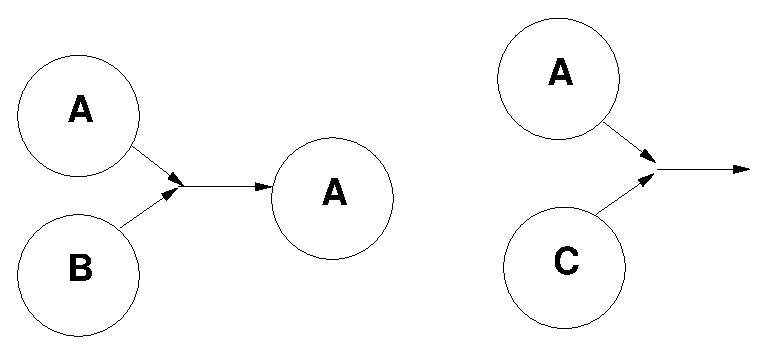
\includegraphics[width=1\columnwidth]{cham1a}%
\end{minipage}\hfill{}

~\\

\begin{itemize}
\item Define molecules \texttt{\textcolor{blue}{\scriptsize{}a}}, \texttt{\textcolor{blue}{\scriptsize{}b}},
\texttt{\textcolor{blue}{\scriptsize{}c}}, ... and arbitrary chemical
laws
\item Inject some molecules into the ``soup''
\item The runtime system evolves the soup \emph{concurrently}
\end{itemize}
\end{frame}

\begin{frame}{Join Calculus in a nutshell}


\framesubtitle{``Better concurrency through chemistry''}

Translating the ``chemical metaphor'' into practice:~\\
~

\fbox{\begin{minipage}[c][1\totalheight][t]{0.5\columnwidth}%
\begin{itemize}
\item Each molecule carries a \textbf{value} 
\item Each reaction computes a ``molecule-valued'' \textbf{expression}
that depends on input values
\item Resulting molecules are injected back into the soup
\item Reactions start concurrently if input molecules are available
\end{itemize}
%
\end{minipage}}\hfill{}%
\begin{minipage}[c][1\totalheight][t]{0.45\columnwidth}%
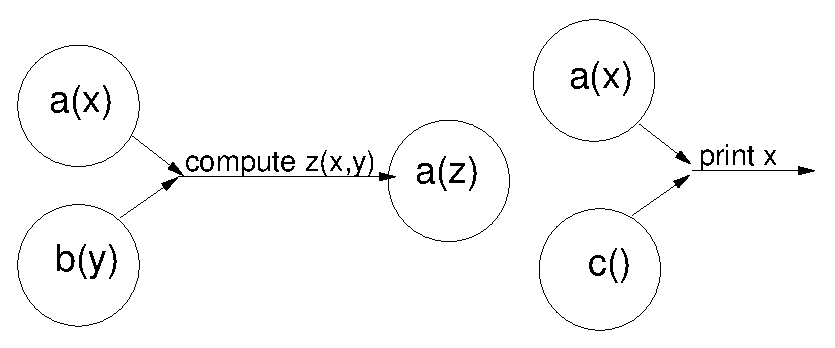
\includegraphics[width=1\columnwidth]{cham2}

~\\
\texttt{\textcolor{blue}{\scriptsize{}join(}}{\scriptsize \par}

\texttt{\textcolor{blue}{\scriptsize{}~ run \{ case }}\texttt{\textbf{\textcolor{blue}{\scriptsize{}a}}}\texttt{\textcolor{blue}{\scriptsize{}(x)
+ }}\texttt{\textbf{\textcolor{blue}{\scriptsize{}b}}}\texttt{\textcolor{blue}{\scriptsize{}(y)
=>}}{\scriptsize \par}

\texttt{\textcolor{blue}{\scriptsize{}~ ~val z = compute\_z(x,y);
}}\texttt{\textbf{\textcolor{blue}{\scriptsize{}a}}}\texttt{\textcolor{blue}{\scriptsize{}(z)
\},}}{\scriptsize \par}

\texttt{\textcolor{blue}{\scriptsize{}~ run \{ case }}\texttt{\textbf{\textcolor{blue}{\scriptsize{}a}}}\texttt{\textcolor{blue}{\scriptsize{}(x)
+ }}\texttt{\textbf{\textcolor{blue}{\scriptsize{}c}}}\texttt{\textcolor{blue}{\scriptsize{}()
=>}}{\scriptsize \par}

\texttt{\textcolor{blue}{\scriptsize{}~ ~ ~ println(x) \} )}}{\scriptsize \par}%
\end{minipage}\hfill{}\\
~\\
When a reaction starts: input molecules disappear, expression is computed,
output molecules are injected
\end{frame}

\begin{frame}{Example: concurrent counter}

Chemical laws:
\begin{itemize}
\item \textcolor{blue}{\scriptsize{}counter(n) + decr() => counter(n-1)}{\scriptsize \par}
\item \textcolor{blue}{\scriptsize{}counter(n) + incr() => counter(n+1)}{\scriptsize \par}
\end{itemize}
``Data stays on the molecules''
\end{frame}

\begin{frame}{Using \texttt{JoinRun}: basic features}


\framesubtitle{Molecule injectors, reaction definitions}

Define \textbf{molecule} \textbf{injectors}:\\
\texttt{\textcolor{blue}{\scriptsize{}val counter = jA{[}Int{]}}}\\
\texttt{\textcolor{blue}{\scriptsize{}val decr = jA{[}Unit{]}}}\\
\texttt{\textcolor{blue}{\scriptsize{}val incr = jA{[}Unit{]}}}{\scriptsize \par}

Declare some \textbf{reactions} using the known molecules:\\
\texttt{\textcolor{blue}{\scriptsize{}val r0 = run \{ case counter(n)
+ decr() => counter(n-1) \}}} \\
\texttt{\textcolor{blue}{\scriptsize{}val r1 = run \{ case counter(n)
+ incr() => counter(n+1) \}}} 

Activate a ``\textbf{join definition}'' and inject some molecules:\\
\texttt{\textcolor{blue}{\scriptsize{}join(r0, r1)}}\\
\texttt{\textcolor{blue}{\scriptsize{}counter(10)}} \textcolor{gray}{\footnotesize{}//
non-blocking side-effect}\\
\texttt{\textcolor{blue}{\scriptsize{}incr()}} \textcolor{gray}{\footnotesize{}//
ditto; now we have}\texttt{\textcolor{gray}{\footnotesize{} counter(11)}}
\\
\texttt{\textcolor{blue}{\scriptsize{}incr()}} \textcolor{gray}{\footnotesize{}//
now we have }\texttt{\textcolor{gray}{\footnotesize{}counter(12)}}{\footnotesize \par}
\begin{itemize}
\item Calling \texttt{\textcolor{blue}{\scriptsize{}counter(10)}} returns
\texttt{\textcolor{blue}{\scriptsize{}Unit}} and injects molecule
as a side-effect
\end{itemize}
\end{frame}

\begin{frame}{Using \texttt{JoinRun}: more features}


\framesubtitle{Blocking vs.~non-blocking molecules}

\textbf{Blocking} molecule:
\begin{itemize}
\item injection will block until reply is received
\item implicitly carries a pseudo-molecule injector: ``reply''
\item when the ``reply'' is injected, the value will be returned to caller
\item Example:\\
\texttt{\textcolor{blue}{\scriptsize{}f(x, replyToF) + c(y) => val
z = ...; replyToF(z) }}{\scriptsize \par}
\end{itemize}
\end{frame}

\begin{frame}{Using \texttt{JoinRun}: more features}


\framesubtitle{Blocking molecules in \texttt{JoinRun}}

Implement blocking access to the value \texttt{\textcolor{blue}{\scriptsize{}x}}
in \texttt{\textcolor{blue}{\scriptsize{}counter(x)}}{\scriptsize \par}

~\\
\texttt{\textcolor{blue}{\scriptsize{}val getN = jS{[}Unit, Int{]}}}\\
\textcolor{gray}{\footnotesize{}// revise the join definition, appending
this reaction:}\\
\texttt{\textcolor{blue}{\scriptsize{}... val r2 = run \{ case counter(x)
+ getN(\_, reply) => reply(x) \}}}\\
\texttt{\textcolor{blue}{\scriptsize{}join(r0, r1, r2)}}\\
\textcolor{gray}{\footnotesize{}// inject non-blocking molecules...
}\\
\textcolor{gray}{\footnotesize{}// now inject the blocking molecule:}\\
\texttt{\textcolor{blue}{\scriptsize{}val x = getN()}}\textcolor{gray}{\footnotesize{}
// blocking call, returns }\texttt{\textcolor{gray}{\footnotesize{}Int}}\\

\end{frame}

\begin{frame}{\texttt{JoinRun}: Examples I}


\framesubtitle{First benchmark: Counting to zero}

Concurrent non-blocking counter:\\
\texttt{\textcolor{blue}{\scriptsize{}~}}\\
\texttt{\textcolor{blue}{\scriptsize{}val c = ja{[}Int{]}(\textquotedbl{}counter\textquotedbl{})}}{\scriptsize \par}

\texttt{\textcolor{blue}{\scriptsize{}val g = js{[}Unit,Int{]}(\textquotedbl{}getValue\textquotedbl{})}}{\scriptsize \par}

\texttt{\textcolor{blue}{\scriptsize{}val d = ja{[}Unit{]}(\textquotedbl{}decr\textquotedbl{})}}{\scriptsize \par}

\texttt{\textcolor{blue}{\scriptsize{}val f = js{[}LocalDateTime,
Long{]}(\textquotedbl{}finished\textquotedbl{})}}{\scriptsize \par}

\texttt{\textcolor{blue}{\scriptsize{}~}}{\scriptsize \par}

\texttt{\textcolor{blue}{\scriptsize{}join(}}{\scriptsize \par}

\texttt{\textcolor{blue}{\scriptsize{}~ ~run \{ case c(0) + f(t,
reply) =>}}{\scriptsize \par}

\texttt{\textcolor{blue}{\scriptsize{}~ ~~ ~val elapsed = t.until(LocalDateTime.now,
ChronoUnit.MILLIS)}}{\scriptsize \par}

\texttt{\textcolor{blue}{\scriptsize{}~ ~~ ~reply(elapsed) \},}}{\scriptsize \par}

\texttt{\textcolor{blue}{\scriptsize{}~ ~run \{ case g(\_,reply)
+ c(n) => c(n) + reply(n) \},}}{\scriptsize \par}

\texttt{\textcolor{blue}{\scriptsize{}~ ~run \{ case c(n) + d(\_)
if n > 0 => c(n-1) \}}}{\scriptsize \par}

\texttt{\textcolor{blue}{\scriptsize{})}}{\scriptsize \par}

\texttt{\textcolor{blue}{\scriptsize{}val initialTime = LocalDateTime.now}}{\scriptsize \par}

\texttt{\textcolor{blue}{\scriptsize{}c(1000)}}{\scriptsize \par}

\texttt{\textcolor{blue}{\scriptsize{}(1 to 1000).foreach\{ \_ =>
d() \}}}{\scriptsize \par}

\texttt{\textcolor{blue}{\scriptsize{}val result = f(initialTime)}}{\scriptsize \par}
\end{frame}

\begin{frame}{\texttt{JoinRun}: Examples II}


\framesubtitle{Options, Futures, and Map/Reduce}

Future with blocking poll (``\texttt{\textcolor{blue}{\scriptsize{}get}}''):\\
\texttt{\textcolor{blue}{\scriptsize{}fut( (f,x) ) => finished( f(x)
)}}\\
\texttt{\textcolor{blue}{\scriptsize{}get(\_, r) + finished(fx) =>
r(fx)}}\\
~\\
~

Map/Reduce:\\
\texttt{\textcolor{blue}{\scriptsize{}\{ case res(list) + c(s) =>
res(s::list) \} }}\\
\texttt{\textcolor{blue}{\scriptsize{}\{ case get(\_, reply) + res(list)
=> reply(list) \}}}\\
\texttt{\textcolor{blue}{\scriptsize{}res(Nil)}} \\
\texttt{\textcolor{blue}{\scriptsize{}Seq(1,2,3).foreach(x => c(x{*}2))}}\\
\texttt{\textcolor{blue}{\scriptsize{}get()}}\textcolor{gray}{\footnotesize{}
// this returned Seq(4,6,2) in one test}{\footnotesize \par}
\end{frame}

\begin{frame}{\texttt{JoinRun}: Examples III}


\framesubtitle{Five Dining Philosophers}

Philosophers \texttt{\textcolor{blue}{\scriptsize{}1, 2, 3, 4, }}\textcolor{blue}{\scriptsize{}5};
forks \texttt{\textcolor{blue}{\scriptsize{}f12, f23, f34, f45, f51}}.
\begin{lyxcode}
\textsf{\textcolor{gray}{\footnotesize{}//~...~some~declarations~omitted~for~brevity}}{\footnotesize \par}

\textcolor{blue}{\scriptsize{}join~(}{\scriptsize \par}

\textcolor{blue}{\scriptsize{}~~run\{~case~t1(\_)~=>~wait();~h1()~\},}{\scriptsize \par}

\textcolor{blue}{\scriptsize{}~~run\{~case~t2(\_)~=>~wait();~h2()~\},}{\scriptsize \par}

\textcolor{blue}{\scriptsize{}~~run\{~case~t3(\_)~=>~wait();~h3()~\},}{\scriptsize \par}

\textcolor{blue}{\scriptsize{}~~run\{~case~t4(\_)~=>~wait();~h4()~\},}{\scriptsize \par}

\textcolor{blue}{\scriptsize{}~~run\{~case~t5(\_)~=>~wait();~h5()~\},}{\scriptsize \par}

\textcolor{blue}{\scriptsize{}~~run\{~case~h1(\_)~+~f12(\_)~+~f51(\_)~=>~wait();~t1()~+~f12()~+~f51()~\},}{\scriptsize \par}

\textcolor{blue}{\scriptsize{}~~run\{~case~h2(\_)~+~f23(\_)~+~f12(\_)~=>~wait();~t2()~+~f23()~+~f12()~\},}{\scriptsize \par}

\textcolor{blue}{\scriptsize{}~~run\{~case~h3(\_)~+~f34(\_)~+~f23(\_)~=>~wait();~t3()~+~f34()~+~f23()~\},}{\scriptsize \par}

\textcolor{blue}{\scriptsize{}~~run\{~case~h4(\_)~+~f45(\_)~+~f34(\_)~=>~wait();~t4()~+~f45()~+~f34()~\},}{\scriptsize \par}

\textcolor{blue}{\scriptsize{}~~run\{~case~h5(\_)~+~f51(\_)~+~f45(\_)~=>~wait();~t5()~+~f51()~+~f45()~\}}{\scriptsize \par}

\textcolor{blue}{\scriptsize{})}{\scriptsize \par}

\textcolor{blue}{\scriptsize{}t1()~+~t2()~+~t3()~+~t4()~+~t5()}{\scriptsize \par}

\textcolor{blue}{\scriptsize{}f12()~+~f23()~+~f34()~+~f45()~+~f51()}{\scriptsize \par}
\end{lyxcode}
\end{frame}

\begin{frame}{Additional features of \texttt{JoinRun}}

\framesubtitle{More bells and whistles}
\begin{itemize}
\item Per-reaction thread pools:\\
\texttt{\textcolor{blue}{\scriptsize{}val tp1 = new JReactionPool(threads
= 1)}}\\
\texttt{\textcolor{blue}{\scriptsize{}val tp8 = new JReactionPool(threads
= 8)}}\\
\texttt{\textcolor{blue}{\scriptsize{}join(}}\\
\texttt{\textcolor{blue}{\scriptsize{} ~ run \{ case a(x) + b(y)
=> ... \} onThreads tp1,}}\\
\texttt{\textcolor{blue}{\scriptsize{} ~ run \{ case a(x) + c(y)
=> ... \} onThreads tp8}}\\
\texttt{\textcolor{blue}{\scriptsize{})}}\\
\medskip{}
\item Auto-resume failed reactions:\\
\texttt{\textcolor{blue}{\scriptsize{}run \{ case a(x) + b(y) => if
(bad) throw new Exception(); ... \} }}\\
\texttt{JoinRun} will reinject input molecules if exception is thrown
\end{itemize}
\end{frame}

\begin{frame}{Roadmap for \texttt{JoinRun}}

\framesubtitle{Need still more bells and whistles}
\begin{itemize}
\item Graceful global shutdown
\item Resilience to failure in join definitions
\item Runtime diagnostics, health monitoring
\item Run on a cluster (``Distributed Join Calculus'')
\end{itemize}
What else is needed for industry-readiness?
\end{frame}

\begin{frame}{\texttt{JoinRun}: Examples IV}


\framesubtitle{Concurrent merge-sort: chemistry}

The \texttt{\textcolor{blue}{\scriptsize{}mergesort}} molecule is
``recursive'':
\begin{itemize}
\item receives the upper-level ``\texttt{\textcolor{blue}{\scriptsize{}sortedResult}}''
molecule
\item defines its own ``\texttt{\textcolor{blue}{\scriptsize{}sorted}}''
molecules in \emph{local scope}
\item emits upper-level ``\texttt{\textcolor{blue}{\scriptsize{}sortedResult}}''
when done
\end{itemize}
\begin{lyxcode}
\textcolor{blue}{\scriptsize{}mergesort(~(arr,~sortedResult)~)~=>}{\scriptsize \par}

\textcolor{blue}{\scriptsize{}~~~~~~~val~(part1,~part2)~=~arr.splitAt(arr.length/2)}{\scriptsize \par}

\textcolor{blue}{\scriptsize{}~~~~~~~sorted1(x)~+~sorted2(y)~=>~sortedResult(~arrayMerge(x,y)~)}{\scriptsize \par}

\textsf{\textcolor{gray}{\footnotesize{}~~~~~~~//~inject~lower-level~mergesort}}{\footnotesize \par}

\textcolor{blue}{\scriptsize{}~~~~~~~mergesort(part1,~sorted1)~+~mergesort(part2,~sorted2)}{\scriptsize \par}

\end{lyxcode}
\end{frame}

\begin{frame}{\texttt{JoinRun}: Examples IV}


\framesubtitle{Concurrent merge-sort: \texttt{JoinRun} code}
\begin{lyxcode}
\textcolor{blue}{\scriptsize{}val~mergesort~=~new~JA{[}(Array{[}T{]},~JA{[}Array{[}T{]}{]}){]}}{\scriptsize \par}

\textcolor{blue}{\scriptsize{}join(}{\scriptsize \par}

\textcolor{blue}{\scriptsize{}~~run~\{~case~mergesort((arr,~sortedResult))~=>}{\scriptsize \par}

\textcolor{blue}{\scriptsize{}~~~~if~(arr.length~<=~1)~sortedResult(arr)}{\scriptsize \par}

\textcolor{blue}{\scriptsize{}~~~~~~else~\{}{\scriptsize \par}

\textcolor{blue}{\scriptsize{}~~~~~~~~val~sorted1~=~new~JA{[}Array{[}T{]}{]}}{\scriptsize \par}

\textcolor{blue}{\scriptsize{}~~~~~~~~val~sorted2~=~new~JA{[}Array{[}T{]}{]}}{\scriptsize \par}

\textcolor{blue}{\scriptsize{}~~~~~~~~join(}{\scriptsize \par}

\textcolor{blue}{\scriptsize{}~~~~~~~~~~run~\{~case~sorted1(x)~+~sorted2(y)~=>~sortedResult(arrayMerge(x,y))~\}}{\scriptsize \par}

\textcolor{blue}{\scriptsize{}~~~~~~~~)}{\scriptsize \par}

\textcolor{blue}{\scriptsize{}~~~~~~~~val~(part1,~part2)~=~arr.splitAt(arr.length/2)}{\scriptsize \par}

\textcolor{blue}{\scriptsize{}~~~~~~~~}\textsf{\textcolor{gray}{\footnotesize{}//~inject~lower-level~mergesort}}{\footnotesize \par}

\textcolor{blue}{\scriptsize{}~~~~~~~~mergesort(part1,~sorted1)~+~mergesort(part2,~sorted2)}{\scriptsize \par}

\textcolor{blue}{\scriptsize{}~~~~\}}{\scriptsize \par}

\textcolor{blue}{\scriptsize{}~~\})}{\scriptsize \par}
\end{lyxcode}
\end{frame}

\begin{frame}{Join Calculus in the wild}

\begin{itemize}
\item Previous implementations:
\begin{itemize}
\item Funnel {[}\href{http://lampwww.epfl.ch/funnel/}{M. Odersky et al., 2000}{]}
\item Join Java {[}\href{http://www.vonitzstein.com/Project_JoinJava.html}{von Itzstein et al., 2001-2005}{]}
\item JOCaml  (\href{http://jocaml.inria.fr}{jocaml.inria.fr}) {[}\href{http://research.microsoft.com/en-us/um/people/fournet/papers/jocaml-afp4-summer-school-02.pdf}{Fournet et al.�2003}{]}
\item ``Join in Scala'' compiler patch {[}\href{http://lampwww.epfl.ch/~cremet/misc/join_in_scala/index.html}{V. Cremet 2003}{]}
\item Joins library for .NET {[}\href{http://research.microsoft.com/en-us/um/people/crusso/joins/}{P. Crusso 2006}{]}
\item ScalaJoins {[}\href{http://lampwww.epfl.ch/~phaller/joins/index.html}{P. Haller 2008}{]}
\item Joinads (F\#, Haskell) {[}\href{https://www.microsoft.com/en-us/research/publication/joinads-a-retargetable-control-flow-construct-for-reactive-parallel-and-concurrent-programming/}{Petricek and Syme 2011}{]}
\item ScalaJoin {[}\href{https://github.com/Jiansen/ScalaJoin}{J. He 2011}{]}
\item \href{https://github.com/winitzki/CocoaJoin}{CocoaJoin (iOS)}, \href{https://github.com/winitzki/AndroJoin}{AndroJoin (Android)}
{[}S.W.\texttt{\textcolor{blue}{\scriptsize{}~}}2013{]}
\end{itemize}
\item \href{https://github.com/winitzki/joinrun-scala}{JoinRun} -{}- a
new JC prototype in Scala (this talk)
\begin{itemize}
\item Better syntax, more checks of code sanity
\item (Some) automatic fault tolerance
\item Fair scheduling of reactions
\item Can use thread pools or Akka event-driven actor pools
\end{itemize}
\end{itemize}
\end{frame}

\begin{frame}{Other approaches to concurrency}

\begin{itemize}
\item STM
\item \texttt{Erlang's} message-passing $\approx$ Akka's ``actors''
\item CSP / \texttt{Go} language
\item $\pi$-calculus, \textbf{join calculus} (academic so far)
\end{itemize}
\end{frame}

\begin{frame}{Comparison: Join Calculus vs. Actor model}

\hfill{}Reaction $\approx$ actor\hfill{}Injected molecule $\approx$
message to actor\hfill{}

Actors: 
\begin{itemize}
\item need to be created and managed explicitly
\item will process one message at a time
\item typically hold mutable state 
\end{itemize}
Reactions:
\begin{itemize}
\item autostart when required input molecules are available
\item many reactions can start at once, automatically concurrent
\item immutable, stateless, and type-safe
\item all reactions are defined statically, but locally scoped
\end{itemize}
\end{frame}

\begin{frame}{And I thought ``actors'' were easy...}

Akka's \href{http://doc.akka.io/docs/akka/current/scala/actors.html}{documentation for the Actor class}:
\texttt{\footnotesize{}\bigskip{}
}

\texttt{\footnotesize{}Actor}{\footnotesize{}, }\texttt{\footnotesize{}ActorSystem}{\footnotesize{},
}\texttt{\footnotesize{}Props}{\footnotesize{} (but note the 4 edge
cases and 2 warnings)}{\footnotesize \par}

\texttt{\footnotesize{}Actor's}{\footnotesize{} companion object;
}\texttt{\footnotesize{}ActorRef}{\footnotesize \par}

\texttt{\footnotesize{}inbox}{\footnotesize{}, }\texttt{\footnotesize{}self}{\footnotesize{},
}\texttt{\footnotesize{}sender}{\footnotesize{}, }\texttt{\footnotesize{}context}{\footnotesize{},
}\texttt{\footnotesize{}supervisorStrategy}{\footnotesize{}, }\texttt{\footnotesize{}watch}{\footnotesize \par}

\texttt{\footnotesize{}Actor}{\footnotesize{} lifecycle, }\texttt{\footnotesize{}Actor}{\footnotesize{}
selection}{\footnotesize \par}

\texttt{\footnotesize{}send}{\footnotesize{}, }\texttt{\footnotesize{}receive}{\footnotesize{},
}\texttt{\footnotesize{}receive}{\footnotesize{} timeout, }\texttt{\footnotesize{}forward}{\footnotesize \par}

\texttt{\footnotesize{}Future}{\footnotesize{}, }\texttt{\footnotesize{}pipeTo}{\footnotesize \par}

{\footnotesize{}exceptions, exceptions vs.~Future callbacks, }\texttt{\footnotesize{}andThen}{\footnotesize \par}

\texttt{\footnotesize{}stop}{\footnotesize{}, }\texttt{\footnotesize{}gracefulStop}{\footnotesize{},
}\texttt{\footnotesize{}PoisonPill}{\footnotesize{}, }\texttt{\footnotesize{}Kill}{\footnotesize \par}

\texttt{\footnotesize{}become}{\footnotesize{}, }\texttt{\footnotesize{}unbecome}{\footnotesize{},
}\texttt{\footnotesize{}upgrade}{\footnotesize{}, }\texttt{\footnotesize{}stash}{\footnotesize \par}

\texttt{\footnotesize{}\bigskip{}
}

This was item 1 in the Actors documentation.

There are 14 further items...
\end{frame}

\begin{frame}{Everything you need to know about JC...}


\framesubtitle{... but were afraid to ask}

Most descriptions of JC use the ``message/channel'' metaphor... 

\texttt{\footnotesize{}\bigskip{}
}{\footnotesize \par}
\begin{center}
\begin{tabular}{|c|c|c|}
\hline 
``Chemistry'' & JC terminology & \texttt{JoinRun}\tabularnewline
\hline 
\hline 
molecule & message on channel & \texttt{\textcolor{blue}{\footnotesize{}a(123)}}\textcolor{gray}{\footnotesize{}
// side effect}\tabularnewline
\hline 
injector & channel (port) name & \texttt{\textcolor{blue}{\footnotesize{}val a : JA{[}Int{]}}}\tabularnewline
\hline 
blocking injector & blocking channel & \texttt{\textcolor{blue}{\footnotesize{}val q : JS{[}Int{]}}}\tabularnewline
\hline 
reaction & process & \texttt{\textcolor{blue}{\footnotesize{}run \{ case a(x) + ... \}}}\tabularnewline
\hline 
injecting a molecule & sending a message & \texttt{\textcolor{blue}{\footnotesize{}a(123)}}\textcolor{gray}{\footnotesize{}
// side effect}\tabularnewline
\hline 
join definition & join definition & \texttt{\textcolor{blue}{\footnotesize{}join(r1, r2, ...)}}\tabularnewline
\hline 
\end{tabular}
\par\end{center}

\end{frame}

\begin{frame}{Conclusions and outlook}

\begin{itemize}
\item Join Calculus = declarative, purely functional concurrency
\item Similar to ``Actors'', but far easier and ``more purely functional''
\item Very little known, and very little used in practice
\item Existing literature is not suitable as introduction to practical use
\item A new Scala implementation, \href{https://github.com/winitzki/joinrun-scala}{JoinRun},
is in the works
\end{itemize}
\end{frame}

\end{document}
